\documentclass[11pt]{article}
\usepackage[utf8]{inputenc}
\usepackage[T1]{fontenc}
\usepackage{amsmath}
\usepackage{amsfonts}
\usepackage{amssymb}
\usepackage[version=4]{mhchem}
\usepackage{stmaryrd}
\usepackage{graphicx}
\usepackage[export]{adjustbox}
\graphicspath{ {./images/} }

\begin{document}
Credit Default Swaps

By far the most important development for credit derivatives is the credit default swap. A credit default swap (CDS) is an insurance-like bilateral contract in which the buyer pays a periodic fee (analogous to an insurance premium) to the seller in exchange for a contingent payment from the seller if a credit event occurs with respect to an underlying credit-risky asset. A CDS may be negotiated on any of a variety of credit-risky investments, primarily corporate bonds.

\section*{Credit Default Swaps and Total Return Swaps}
There are two primary types of swaps involving credit risk. The first type, by far the more predominant, is the CDS. In a CDS, the credit protection buyer pays a periodic premium on a predetermined amount (the notional amount) in exchange for a contingent payment from the credit protection seller if a specified credit event occurs. The credit protection buyer typically uses the payment to hedge losses suffered from the specified credit event. The credit protection seller receives a periodic premium in exchange for delivering a contingent payment to the credit protection buyer if a specified credit event occurs. ${ }^{1}$ In dealing with credit derivatives, practitioners often shorten the terms credit protection buyer and credit protection seller to protection buyer and protection seller, or even simply buyer and seller. This session transitions from the longer terms to the shorter terms as the reader is assumed to be developing better familiarity with the terminology and concepts.

The next exhibit demonstrates a CDS. In this illustration, the credit protection buyer is assumed to hold a cash position in a credit-risky asset and is using a CDS to purchase credit protection. In the next exhibit, the credit risk of the underlying risky asset is transferred from the credit protection buyer to the credit protection seller. The credit protection seller may be interested in bearing the credit risk for the potential rewards or may hedge the credit risk away, using, for example, another credit derivative. Subsequent sections discuss CDSs in detail.

\begin{center}
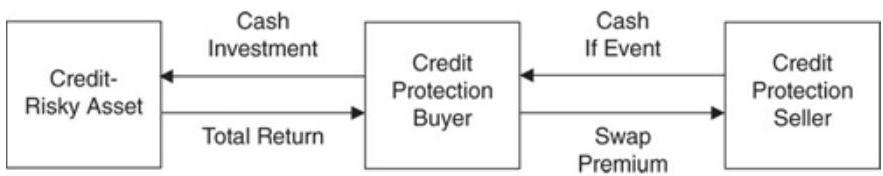
\includegraphics[max width=\textwidth]{2024_04_09_87c8b6247d8feabc3893g-2(1)}
\end{center}

\section*{Credit Default Swap}
A variation on the CDS is a total return swap with a credit-risky reference asset. In a total return swap, the credit protection buyer, typically the owner of the credit risky asset, passes on the total return of the asset to the credit protection seller in return for a certain payment. Thus, the credit protection buyer gives up the uncertain returns of the credit-risky asset in return for a certain payment from the credit protection seller. The credit protection seller now receives both the upside and the downside of the return associated with the credit-risky asset. The credit protection seller takes on all of the economic risk of the underlying asset, just as if that asset were on the balance sheet or in the investment portfolio. The Total Return Swap exhibit on a Risky Asset demonstrates this total return swap.

\begin{center}
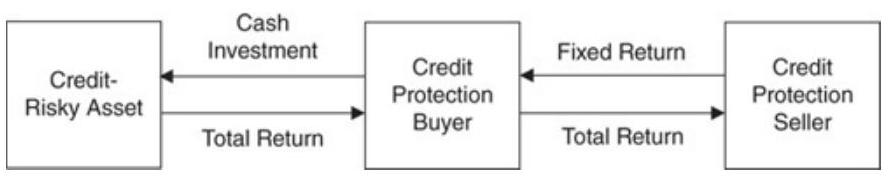
\includegraphics[max width=\textwidth]{2024_04_09_87c8b6247d8feabc3893g-2}
\end{center}

\section*{Total Return Swap on a Risky Asset}
The left sides of both the exhibits, Credit Default Swap and Total Return Swap on a Risky Asset are the same and illustrate the idea that the credit protection buyer is assumed in these examples to own the underlying asset that contains the credit risk (e.g., a risky corporate bond). Comparison of the two exhibits illustrates the essential differences between a CDS and a total return swap on the same credit risk. In the case of a CDS, the credit protection buyer makes fixed payments, known as the swap premium, to the credit protection seller. If the credit experiences a trigger event (e.g., a default), the credit protection buyer receives cash from the credit protection seller. In the case of a total return swap, the credit protection buyer makes payments to the credit protection seller based on the total market return of the underlying asset. The total market return is composed of any coupon payments and any change in the underlying bond's market price. The credit protection buyer receives a payment from the credit protection seller that may vary with interest rates but does not vary based on the performance of the same credit risk.

CDSs and total return swaps on credit-risky assets are used to transfer risk. For example, a bank may use a CDS to hedge the credit exposure on its balance sheet, such as its exposure to a particular corporate borrower or to an industry that the bank believes is geared for difficult times. The bank can reduce its exposure to the credit risk of one or more of its customers, in most cases without the knowledge or consent of the customers.

CDSs are very flexible. For instance, a CDS may state in its contract the exact amount of insurance payment in the event of a credit event. Alternatively, a CDS may be structured so that the amount of the swap payment by the credit protection seller is determined after the credit event. Usually, the payment by the credit protection seller in the event of a credit event is determined by the market value of the referenced asset after the credit event has occurred. In total return swaps, there is no need to specify the events that lead to payments, since payments are driven by market values.

\section*{Mechanics of a Credit Default Swap}
The CDS market is contract driven. This means that each CDS is a privately negotiated transaction between the credit protection buyer and the credit protection seller. Fortunately, the ISDA, the primary industry body for derivatives documentation, has established standardized terms for CDSs. These terms are not mandated for use but are available to market participants and are used as a framework for negotiating a deal. This section provides some detail regarding the standard ISDA agreement. The standard ISDA agreement serves as a template to negotiated credit agreements that contains provisions commonly used by market participants. The standard ISDA agreement provides specifications relating to the following five aspects of the deal:

\begin{enumerate}
  \item CDS spread: The CDS spread or CDS premium is paid by the credit protection buyer to the credit protection seller and is quoted in basis points per annum on the notional value of the CDS. The CDS spread is not a credit yield spread but a price or rate quote for buying credit insurance. Typically, the price of this credit insurance is paid quarterly by the protection buyer.

  \item Contract size: ISDA does not impose any limits on size or length of term of a CDS; this is up to the negotiation of the parties involved. The notional value of most CDSs falls in the range of $\$ 20$ million to $\$ 200$ million, with a tenor (term) of three to five years.

  \item Trigger events: This is the heart of every CDS transaction. Trigger events determine when the credit protection seller must make a payment to the credit protection buyer. Both sides to a CDS negotiate these terms intensely. The broader the definition of a trigger event, the more likely cash will flow from the protection seller to the protection buyer and the higher the appropriate spread will be. The ISDA agreement provides for seven kinds of potential trigger events; the parties to a CDS are welcome to add more, although the seven events identified by ISDA cover virtually all types of credit events:

  \item Bankruptcy. A filing for bankruptcy is typically associated with a company's inability to pay its debt.

  \item Failure to pay. Although a company may not be in bankruptcy yet, it may not be able to meet its debt obligations as they come due.

  \item Restructuring. This is any form of debt restructuring that is disadvantageous to a holder of the referenced credit. Restructuring is a fuzzy term, and ISDA attempts to clarify this part of the standard contract by offering the following four options for the parties to consider: no restructuring, full restructuring, modified restructuring (which limits resulting obligations to bonds maturing in less than 30 months), and modified-modified restructuring (which is less strict than modified restructuring because resulting bonds can have maturities of up to 60 months).

  \item Obligation acceleration. All bond and loan covenants contain provisions that accelerate the repayment of the loan or bond if the credit quality of the borrower begins to deteriorate due to a number of events, such as a failure to pay, a bankruptcy (which ISDA covers independently), or a ratings downgrade.

  \item Obligation default. This is any failure to meet a condition in the bond or loan covenant that would put the borrower in breach of the covenant. It could be something like the failure to maintain a sufficient current ratio or a minimum interest earnings coverage ratio.

  \item Repudiation/moratorium. This is most frequently associated with sovereign or emerging markets debt. It is simply a refusal by the sovereign government to repay its debt as it comes due or even an outright rejection of its debt obligations.

  \item Government intervention. A government's action or announcement reduces required payments or reduces the priority of making payments.

  \item Settlement. If a credit event occurs, settlement can be made either with a cash payment or with a physical settlement. In a cash settlement, the credit protection seller makes the credit protection buyer whole by transferring to the buyer an amount of cash based on the contract. The settlement price can sometimes be the present value of the contractual cash flows over its remaining life, or it may be determined through auction processes. Cash settlement does not occur as frequently as one might expect, because it is difficult to agree on a good market-based measure of the loss. Therefore, most CDSs use physical settlement upon the occurrence of a credit event. Under physical settlement, the credit protection seller purchases the impaired loan or bond from the credit protection buyer at par value. The credit-risky asset is physically transferred to the credit protection seller's balance sheet, and the face or par value of the bond is transferred to the protection buyer from the protection seller.

  \item Delivery. Within particular limits, the credit protection buyer has a choice of assets that can be delivered for physical settlement. This raises the issue of which of those assets is cheapest to deliver. The concept of multiple deliverable assets is common throughout derivatives and provides an option to the holder of the short option position that should be reflected in the contract's price or terms. Deliverables can include direct obligations of the referenced entity, such as corporate bonds or bank loans; obligations of a subsidiary of the referenced entity if the subsidiary is at least 50\% owned by the referenced entity (sometimes referred to as qualifying affiliate guarantees); and obligations of a third party that the referenced entity may have guaranteed (known as qualifying guarantees). Note that physical settlement can create problems if there is an insufficient supply of assets to deliver, possibly because the notional value of an outstanding CDS exceeds the principal value of the underlying bonds.

\end{enumerate}

Keep in mind that although ISDA provides standard terms, the parties to a CDS can negotiate any and all terms, plus add their own if they both wish. The main point is that the standardization of CDS terms has provided the infrastructure for the huge growth of the credit derivatives market.

As this example shows, four major terms define a CDS:

\begin{enumerate}
  \item Credit reference: CDS contracts specify a referenced asset. The referenced asset (also called the referenced bond, referenced obligation, or referenced credit) is the underlying security on which the credit protection is provided. Following a credit event, particular qualifying bonds are deliverable. Typically, a senior unsecured bond is the reference entity, but bonds at other levels of the capital structure may be referenced.

  \item Notional amount. CDS contracts specify the amount of credit risk being transferred. This amount, agreed on by both the protection buyer and the protection seller, is analogous to the principal value of a cash bond.

  \item CDS spread: This is the annual payment rate, quoted in basis points. Payments are paid quarterly and accrue on an actual/360-day basis. The spread is also called the fixed rate, coupon, premium, or price.

  \item CDS maturity: Typically, CDS contracts expire on the 20th of March, June, September, or December. The five-year contract is usually the most common and most liquid.

\end{enumerate}

The economics of the CDS in the previous example can be viewed from the perspective of the bank. Suppose that the bank owned $\$ 20$ million in face value of the referenced credit (bond). What yield would that bond be expected to offer relative to the riskless rate, given that a CDS was available at a spread of $2 \%$ ? The answer is that the yield on the risky debt must exceed the yield on riskless debt of similar maturity by approximately the same rate as the CDS spread, $2 \%$. Thus, in the example, the bank earns $2 \%$ more than the riskless rate (i.e., earns the credit spread) by holding the risky bond, then lays off all that risk by paying a $2 \%$ CDS spread. The bank as a protection buyer hedges the credit risk and earns a return equal to the riskless rate. In practice, the CDS spread can differ from the yield spread due to factors such as the counterparty risk of the CDS.

\section*{Valuing CDS Contracts}
Generally, CDSs and other swaps are entered into without immediate cash payments from either side and are viewed as having near zero market values to each side at inception. This is because the present value of the expected premiums paid by the CDS buyer should be approximately equal to the present value of the expected payments to be made by the CDS seller. As time passes, the risk of the referenced asset may change, general credit conditions may change, and market prices and yields may change. Thus, the value of a CDS should be expected to change through time.

The process of altering the value of a CDS in the accounting and financial systems of the CDS parties is known as a mark-to-market adjustment. Investors perform a mark-to-market (MTM) adjustment to the value of CDS contracts for three primary reasons: financial reporting, realizing economic gains or losses, and managing collateral.

If the market premium moves wider than the contract premium, a protection buyer experiences an MTM gain because the protection was bought more cheaply than is currently available in the market. But if the market premium tightens, the protection seller experiences an MTM gain (and the protection buyer experiences an MTM loss). Calculating a CDS MTM adjustment is essentially the same as calculating the cost of entering into an offsetting transaction.

Suppose an investor bought five-year protection through a CDS at a spread of 100 basis points (bps) per year. One year later, the spread for the same protection (with four remaining years) has widened to 120 bps. The investor would then have an MTM gain, since the protection, for which the investor is paying $100 \mathrm{bps}$ per year, now has a market value of 120 bps per year. To calculate this MTM amount, one can assume a hypothetical offsetting trade in which the investor sells identical protection at $120 \mathrm{bps}$ for four years to hedge the position. This would leave a fixed residual cash flow of $20 \mathrm{bps}$ per year for up to four years in favor of the investor. However, this hypothetical annuity would terminate prior to four years if a triggering credit event occurred. The present value of this annuity, adjusted for the possibility of termination prior to four years, is the MTM amount.

\section*{Unwinding a CDS Transaction}
A party to an OTC derivative that decides to unwind a position (perhaps to monetize the gains or losses or because the credit exposure of the CDS is no longer desired) typically has three alternatives. First, the party can enter into an offsetting transaction. Second, the party can enter into a novation, also known as an assignment. A novation or an assignment is when one party to a contract reaches an agreement with a third party to take over all rights and obligations to a contract. Third, the parties to the OTC contract can agree to terminate the contract (with or without a payment from one party to the other). Details of each of these alternatives follow:

\begin{enumerate}
  \item Entering an offsetting position: The CDS exposure can be offset with a position either in another CDS contract or in one of the underlying deliverable obligations. If the offset is in the underlying bonds, the investor has to separately hedge out the residual interest rate risk. If the offset is with another CDS contract, it most likely results in counterparty risk and a spread differential reflecting changes in the market spread since the first CDS position was established.

  \item Assigning the contract. Investors may be able to locate a dealer or another entity that will take over the rights and obligations of the contract with or without a cash payment from one party to the other. If so, the investor can assign (i.e., novate) the contract. The original counterparty must give permission for assignment because of the counterparty risk present in any CDS contract. The ISDA master agreement requires a transferrer to obtain prior written consent from the remaining party before a novation takes place. Due to potential exposures of CDS parties to the credit risk of the other party, assignments typically occur only when the non-dealer in the contract is replaced by a dealer.

  \item Terminating the contract. The CDS contract can be terminated with mutual consent if necessary by having one of the counterparties pay the other counterparty any lost value from discontinuing the swap. (The valuation of an existing CDS is discussed in a previous section.)

\end{enumerate}

\section*{Participants in Credit Derivatives Markets}
Credit derivatives in general and CDSs in particular have been adopted by virtually all types of financial institutions to take on credit risk, reduce credit risk, or otherwise manage credit risk, or to implement various investment strategies. Although banks remain important players in credit derivatives markets, trends indicate that asset managers are likely to be the major force behind the future growth of these markets. Participants use CDSs for various reasons and follow different trading strategies to hedge risk, increase return, make markets, and reduce funding costs. The following are the main strategies adopted by market participants. ${ }^{2} \mathrm{JPMorgan}$, Credit Derivatives Handbook (New York: Corporate Quantitative Research, 2006); Bank of America, Credit Default Swap Primer (San Francisco: Banc of America Securities, 2008).

\begin{itemize}
  \item Bank trading activities: Major banks serve as market makers in credit derivatives markets and were historically constrained in their ability to provide liquidity because of limits on the amount of credit exposure they could have in one company or sector. The use of more efficient hedging strategies, including credit derivatives, has helped market makers trade more efficiently and employ less capital. Also, CDSs allow market makers to hold their inventory of bonds during a downturn in the credit cycle while remaining neutral in terms of credit risk.
  \item Bank loan portfolios: Banks were once the primary participants in credit derivatives markets. They developed the CDS market to reduce their risk exposure to companies to which they lent money or became exposed through other transactions, thus reducing the amount of capital needed to satisfy regulatory requirements. Banks continue to use credit derivatives for hedging both single-name and broad market credit exposure.
  \item Hedge funds: Since their early participation in credit derivatives markets, hedge funds have continued to increase their presence and the variety of trading strategies in the markets. Whereas the activity of hedge funds was once primarily driven by convertible bond arbitrage, many funds now use CDSs as the most efficient method to buy and sell credit risk. Additionally, hedge funds have been the primary users of relative value trading opportunities and new products that facilitate the trading of credit spread volatility, correlation, and recovery rates.
  \item Other asset managers: Asset managers use credit derivatives markets because they provide opportunities that the managers cannot find in the bond market, such as a particular credit risk with a particular maturity. In addition, credit derivatives markets provide a relatively easy method for avoiding cash sales or overcoming difficulties of short selling. For example, an asset manager might purchase three-year protection to hedge a 10-year bond position whose creditworthiness is under stress but expected to improve if it can survive the next three years. Finally, the emergence of a liquid CDS index market has provided asset managers with a vehicle to efficiently express macro views on the credit markets.
  \item Insurance companies: The participation of insurance companies in credit derivatives markets can be separated into two distinct groups: (1) life insurers and property-casualty companies, and (2) monolines and reinsurers. Life insurers and property-casualty companies typically use CDSs to sell credit protection to\\
enhance the return on their asset portfolios. Monolines (providers of bond guarantees) and reinsurers often sell credit protection as a source of additional premiums and to diversify their portfolios to include credit risk.
  \item Corporations: Operating firms use credit derivatives markets to manage credit exposure to third parties (e.g., accounts receivable). In some cases, the greater liquidity, transparency of pricing, and structural flexibility of the CDS market make it an appealing alternative to credit insurance or factoring arrangements. Some corporations invest in CDS indices and structured credit products as a way to increase expected returns on pension assets or balance sheet cash positions. Finally, corporations are focused on minimizing their funding costs; to this end, many corporate treasurers monitor their own CDS spreads as a benchmark for pricing new bank and bond deals.
\end{itemize}

\section*{Five Motivations for Credit Default Swaps}
The following are five motivations for entering into CDSs:

\begin{enumerate}
  \item Risk decomposition: Credit derivatives provide an efficient way to decompose and separate risks embedded in complex securities. CDS spreads reflect the price to bear pure credit risk. A corporate bond represents a bundle of risks, including interest rate risk, potential callability risk, potential currency risk, credit risk (constituting both the risk of default and the risk of volatility in credit spreads), and liquidity risk. Before the advent of CDSs, the primary way for a bond investor to adjust a credit risk position was to buy or sell that bond, consequently affecting the investor's positions across the entire bundle of risks. Credit derivatives provide a way to manage default risk independently of interest rate risks. Arbitrage strategies can be efficiently implemented using these instruments. For example, convertible arbitrage managers can use CDSs to hedge the credit risk of their convertible positions without affecting the interest rate risk of the portfolio.

  \item Synthetic shorts: Credit derivatives provide an efficient way to hedge credit risk through shorting credit (i.e., taking a position with a value that varies inversely with default). The credit risk exposure of a corporate bond portfolio might be manageable by selling or shorting the bonds. However, bank loans and other credit instruments may turn out to be impossible or at least very costly to short. CDS contracts can be constructed based on those credit risks. Thus, CDSs can allow investors to establish synthetic short positions to hedge or manage specific credit risks or a broad index of credit risks.

  \item Synthetic cash positions: Credit derivatives offer ways to synthetically create loan or bond substitutes through tailor-made credit products. Credit derivatives are OTC instruments that can be tailored to provide investors with various choices for customizing their risk exposures. For example, investors can select maturities to express views about the timing of future credit events. CDS contracts often refer to a senior unsecured bond, but some CDS contracts refer to senior secured and syndicated secured loans. Having CDSs on several components of the same capital structure allows investors to express views on the relative values within a company's capital structure. Credit derivatives can even be used as an alternative to equity derivatives to express a directional view on a firm.

  \item Market linking. The high liquidity of credit derivatives can serve as a source of information that links structurally separate markets. The CDS market often reacts first and facilitates a reflection of revised prices in less liquid markets, such as bond or loan markets. For example, investors buying newly issued convertible debt are exposed to the credit risk in the bond component of the convertible instrument and may seek to hedge this risk using CDSs. As the buyers of convertible bonds purchase protection, the spreads in the CDS market widen. The spread change may occur before the pricing implications of the convertible debt are reflected in bond market spreads. However, the change in CDS spreads may cause bond spreads to widen as investors seek to maintain the value relationship between bonds and CDSs. Thus, the CDS market can serve as an information conduit and as a link between structurally separate markets.

  \item Liquidity during stress: Credit derivatives provide liquidity in times of turbulence in the credit markets. Before the CDS market, a holder of a distressed or defaulted bond often had difficulty selling the bond, even at reduced prices, because cash bond desks are typically long credit risk due to owning an inventory of bonds. As a result, they are often unwilling to purchase bonds and assume more risk in times of market stress. In contrast, credit derivatives desks typically hold an inventory of protection (short credit risk), having bought protection through CDSs. In distressed markets, investors can reduce long credit risk positions by purchasing credit protection through credit derivatives desks, which may be better positioned to sell credit protection and change their inventory position from being short credit risk to being neutral.

\end{enumerate}

\end{document}